\documentclass[12pt,a4paper]{report}
\usepackage[utf8]{inputenc}
\usepackage{amsmath}
\usepackage{amsfonts}
\usepackage{amssymb}
\usepackage{graphicx}
\usepackage{enumitem}
\usepackage[left=2cm, right=2cm, top=4cm, bottom=2cm]{geometry}

\begin{document}
	%Portada
	\begin{titlepage}
		\centering
		{\scshape\LARGE Universidad Nacional Autónoma de México \par}
		\vspace{1cm}
		{\scshape\Large Probabilidad I\par}
		\vspace{1.5cm}
		{\huge\bfseries Tarea V\par}
		\vspace{.5cm}

		{\Large\itshape Alan Ernesto Arteaga Vázquez \par}
		 \vspace{.5cm}
		{\Large\itshape Raúl Llamosas Alvarado \par}
		 \vspace{.5cm}
		{\Large\itshape Edgar Quiroz Castañeda \par}
	    \vspace{.5cm}
		{\Large\itshape Jean Paul Ruiz Melo\par}
		\vspace{.5cm}
		{\Large\itshape Sandra Del Mar Soto Corderi \par}

		\vfill
		 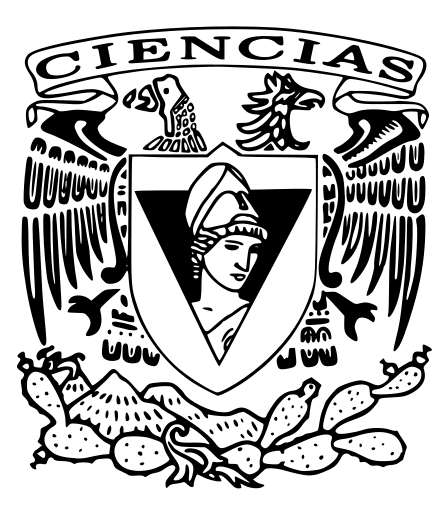
\includegraphics[width=0.5\textwidth]{escudo.png}
		\vfill

		{\large Lunes 26 de octubre del 2018 \par}
	\end{titlepage}

	\pagebreak
	\setlength{\voffset}{-0.75in}
	\setlength{\headsep}{5pt}

	%Ejericios
	\begin{enumerate}
		%1
		\item{
			Suponga de Gage e Itzel participan en un juego, el cual consiste en
			lanzar un dado hasta que alguno de los dos obtenga un 6. Suponga
			que Itzel es la primera en lanzar un dado. ¿Cuál es la probabilidad
			de que Gage gane?
		}

		%2
		\item{
			Considere una variable aleatoria $X$ con una función de densidad
			\[
				f_X(x) = \begin{cases}
					\frac{1-|\frac{x-\alpha}{\beta}|}{\beta},
					$ si $ x \in (\alpha - \beta, \alpha + \beta)\\
					0, $ en otro caso$
				\end{cases}
			\]
			Prueve que $f_X(x)$ es de densidad. Grafíquela.
		}

		%3
		\item{
			\textit{(La paradoja de San Petersburgo, planteada por Nicolás
			Bernoulli en 1728)}.\\
			De acuerdo a la historia, en casino de SanPetersburgo estaba
			dispuesto a ofrecer cualquier tipo de juego siempre que la
			dirección del casino pudiera establecer el precio de la entrara
			que se paga por participar. Se propone el siguiente juego: suponga
			que alguien lanza una moneda balanceada y se reciben $2^n$ pesos
			si cae cara en el $n-$ésimo lanzamiento.\\
			Sea $X$ la ganancia del jugador.
			\begin{enumerate}
				%a
				\item {
				Calcule $\mathbb{E}(X)$.
				}

				%b
				\item {
				¿Estaría dispuesto a liquidar toda la fortuna material que
				posee a cambio de la entrada de este juego?
				}
			\end{enumerate}
		}

		%4
		\item{
			Suponga que se lanzan $n$ dados. Sea $S_n$ la suma de las caras
			obtenidaas al lanzar los $n$ dados.
			\begin{enumerate}
				%a
				\item {
					Encuentre $\mathbb{E}(S_2)$
				}

				%b
				\item {
					Encuentre $\mathbb{E}(S_n)$
				}
			\end{enumerate}
		}

		%5
		\item{
			Sea $Y$ una variable aleatoria con media $\mu > 0$ y varianza
			$\sigma^2 > 0$. Para que valor de $a > 0$ se minimiza
			\begin{enumerate}
				%a
				\item {
					$\mathbb{E}((Y-a)^n)$
				}

				%b
				\item {
					$\mathbb{E}((aY-\frac{1}{a})^2)$
				}
			\end{enumerate}
		}

		%6
		\item{
			Sea $X$ una variable aleatoria con función de densidad
			\[f_X(x) = c \Big(\frac{}{}\Big)^n \mathbb{I}_{\mathbb{N}}(x)\]
			\begin{enumerate}
				%a
				\item {
					Determinar el valor de $c$ para que $f_X$ sea función de
					densidad.
				}

				%b
				\item {
					Encontrar la función generador de momentos $m_X(t)$.
				}
			\end{enumerate}
		}

		%7
		\item{
			Sea $X$ una función de densidad de probabilidad dada por
			\[f_X(x) = \frac{2}{3^x} \mathbb{I}_{\{1, 2, 3, ...\}}(x)\]
			¿Cuál es la probabilidad de que $X$ sea par?
		}

		%8
		\item{
			Sea $X$ variable aleatoria con función de densidad dada por
			\[f_X(x) = \frac{e^{-\frac{x}{2}}}{2}\]
			Con $x > 0$.\\
			Encuentre
			\begin{enumerate}
				%a
				\item {
					$M_X(t)$
				}

				%b
				\item {
					$\mathbb{E}(X)$
				}

				%c
				\item {
					$Var(X)$
				}
			\end{enumerate}
		}

		%9
		\item{
			Demostrar que si $m_X(t)$ es la función generadora de momentos de
			una variable aleatoria $X$, entonces
			\begin{enumerate}
				%a
				\item {
				$\frac{d}{dt}Ln(m_X(t))|_{t = 0} = \mathbb{E}(X)$
				}

				%b
				\item {
				$\frac{d^2}{dt^2}Ln(m_X(t))|_{t = 0} = Var(X)$
				}
			\end{enumerate}
		}

		%10
		\item{
			Conteste
			\begin{enumerate}
				%a
				\item {
					Si $X$ es una variable aleatoria tal que
					$\mathbb{E}(X) = 3$ y $\mathbb{E}(X^2) = 13$, use la
					desigualdad de Chebyshev para determinar una cota inferior
					para $\mathbb{P}(-2 < X < 8)$.
				}

				%b
				\item {
					Sea $X$ una variable aleatoria con función de densidad
					\[
					f_X(x) = \frac{1}{8}\mathbb{I}_{\{-1\}} +
					\frac{6}{8}\mathbb{I}_{\{0\}} +
					\frac{1}{8}\mathbb{I}_{\{1\}}
					\]
					Para $k = 2$, evaluar
					$\mathbb{P}(|X-\mu_X| \geq k\sigma_X)$. Con
					$\mu_X = \mathbb{E}(X)$.\\
					Compare con la cota dada por la desigualdad de Chebyshev.
				}

				%c
				\item {
					Suponga que $X$ es una variable aleatoria con media y
					varianza igual a 20- ¿Qué se puede decir de
					$\mathbb{P}(0 \leq X \leq 40)$?
				}
			\end{enumerate}
		}

		%11
		\item{
			Si $X$ es una variable aleatoria tal que $\mathbb{E}(X) = 3$ y
			$\mathbb{E}(X^2) = 13$, use la desigualdad de Chebyshev para
			determinar una cota mínima para $\mathbb{P}(-2 < X < 8)$.
		}

		%12
		\item{
			Demuestre o dé un contraejemplo
			\begin{enumerate}
				%a
				\item {
					Existe una variable aleatoria $X$ para la cual
					\[\mathbb{P}(\{\omega \in \Omega : E(X) - 2_{\sigma_X} <
					X(\omega) <
					E(X) + 2_{\sigma_X}\}) = \frac{3}{5}\]
				}

				%b
				\item {
					Si $X$ es una variable aleatoria no negativa, entonces
					$\mathbb{E}(X) \leq (\mathbb{E}(X^2))^{\frac{1}{2}}$.
				}
			\end{enumerate}
		}

		%13
		\item{
			Considerese una variable aleatoria $X$ con función de densidad
			$f_X(x) = 2(1-x)\mathbb{I}_{\{0, 1\}}(x)$.\\
			Calcule $\mathbb{E}((X+10)^2)$ y
			$\mathbb{E}\Big(\frac{1}{1-X}\Big)$.
		}

		%14
		\item{
			Un experimento consiste en lanzar dos bolas dentro de cuatro cajas
			de tal forma que cada bola tiene la misma probabilidad de caer en
			cualquier caja. Sea $X$ el número de bolas en la primera caja.
			\begin{enumerate}
				%a
				\item {
					¿Cuál es la función de distribución acumulativa de $X$?
				}

				%b
				\item {
					¿Cuál es la función de densidad de $X$?
				}

				%c
				\item {
					Encontrar $\mathbb{E}(X)$ y $Var(X)$.
				}
			\end{enumerate}
		}

		%15
		\item{
			Sean $a_1, a_2, ..., a_n$ números positivos. Se define
			\begin{align*}
				a_A &= \frac{1}{n}\sum_{i = 0}^{n}{a_i}\\
				a_G &= (\prod_{i = 1}^{n}{a_i})^{\frac{1}{n}}\\
				a_H &= \frac{1}{\frac{1}{n}(\frac{1}{a_1} + ...
				+ \frac{1}{a_n})}
			\end{align*}
			como las medidas aritmética, geométrica y armónica respectivamente.
			Usando la desigualdad de Jenses, demustre que
			\[a_H \leq a_G \leq a_A\]
		}

		%16
		\item{
			Sea $X$ una variable aleatoria no negativa con media 25. ¿Qué puede
			decir de las siguientes cantidades?
			\begin{enumerate}
				%a
				\item {
					$\mathbb{E}(X^3)$
				}

				%b
				\item {
					$\mathbb{E}(\sqrt{X})$
				}

				%c
				\item {
					$\mathbb{E}(log(X))$
				}

				%d
				\item {
					$\mathbb{E}(e^{-X})$
				}
			\end{enumerate}
		}

		%17
		\item{
			\textbf{(OPCIONAL)}\\
			Si $X$ es una variable aleatoria con valor esperado finito,
			entonces
			\[\mathbb{E}(X) = \int_{0}^{\infty}{(1-F_X(x))dx} -
			\int_{-\infty}^{0}{F_X(x)dx}\]
		}

	\end{enumerate}
\end{document}
